\section{Matlab程序设计和GUI设计\scite{2}}
Matlab是一个功能极其强大的数据处理软件,传统的数据分析和处理都是人工计算,在面对一些复杂的计算时,会耗费大量的时间和精力,这就使效率低下。利用计算机进行数据处理,可以将一些重复的、复杂的计算快速准确地进行。利用计算机处理数据,除了可以省时省力外,可以将做过一次数据处理的源码保存下来,下一次进行同类型数据处理的时候可以重复利用。Matlab不仅仅可以进行数据处理,它还支持人机交互界面的设计,也就是Matlab的图形用户界面GUI(Graphical User Interface)。这就使得数据处理变的直观,非专业人士也可以轻松地使用别人开发好的GUI数据处理程序来完成一些数据的分析与处理。
\subsection{Matlab基本操作}
\subsubsection{Matlab的数据基础}
在Matlab软件中,用数组和cell数组的形式来存储任何数据,所有的数据处理是基于变量的操作。
\begin{enumerate}
	\item \textbf{数组}
	\begin{enumerate}
		\item 一维数组
		
		\qquad 数组就是数据的有序集合,一维数组可以看成向量,在处理的时候可以对一组有联系的数据以数组的形式赋值给变量。常用创建数组和获取数组数据的形式如下:
		\begin{lstlisting}
 >> a = [1 2 3 4 5];			% 直接输入创建一维数组,元素可以用空格或逗号隔开
    a = 
		1	2	3	4	5
 >> b = 1:2:9;					% 利用start:step:end 形式创建一维数组
	b =
		1	3	5	7	9
 >> a(3)						% 用变量名加下标的形式获取数组元素
 	ans = 
 		3\end{lstlisting}
		\item 二维数组
		
		\qquad 二维数组可以作为矩阵,在一维数组上增加一具维度,常用的创建和获取数组数据方法如下:
		\begin{lstlisting}
 >> a = [1 2 3;4 5 6;7 8 9]		% 直接输入创建二维数组,用“ ; ”换行
    a = 
    	1	2	3
    	4	5	6
    	7	8	9
 >> b = [1 2 3					% 直接输入创建二维数组,手动换行
 		 4 5 6
 		 7 8 9]
	b = 
	 	1	2	3
	 	4	5	6
	 	7	8	9
 >> a(2,2)						% 用变量名加下标来获取元素,二维数组用行数和列数来确定元素
 	ans = 
 		5\end{lstlisting}
	\end{enumerate}
	\item \textbf{cell数组}
	
	\qquad cell数组也是数组,它也可以是一维和二维,它的特殊之处就是它可以存放任何数据,也就是说它的元素可以是字符串,单个数据,甚至是数组。cell数组的使用方法如下:
	\begin{lstlisting}
 >> a = [1 2 3 4 5];				% 创建一维数组
 >> b = [1 2 3;4 5 6;7 8 9];		% 创建二维数组
 >> c = 'hello';					% 创建字符串
 >> d = {a,b,c}						% 赋值给 cell 数组
 	d = 
 		[1x5 double]	[3x3 double]	'Hello'
 >> d(1)							% 获取元素用“ ( ) ”,不能获取内容
 	ans =
 		[1x5 double]
 >> d{1}							% 获取元素内容用“ { } ”
 	ans =
 		1	2	3	4	5\end{lstlisting}
\end{enumerate}
\subsubsection{Matlab常用函数}
Matlab计算功能之所以强大,是因为它拥有很多的工具箱,里面封装了许多用于处理数据的函数,我们掌握如何使用这些函数,就掌握了Matlab的使用。在误差理论与数据处理中,我们常用的Matlab函数如下表:
\begin{figure}[H]
	\centering
	\begin{tabular}{p{3cm}<{\centering}p{8cm}}
		\toprule
		\textbf{函数}&\multicolumn{1}{c}{\textbf{作用}}	\\
		\midrule
		length(a)	&获取一维数组的长度\\
		size(A)	&获取二维数组的行与列\\
		max(A)	&获取数组A的最大值\\
		min(A)	&获取数组A的最小值\\
		mean(A)	&获取数组A的平均值\\
		sqrt(n)	&获取数值n的算术平方根\\
		std(X)	&获取数据X的标准差\\
		inv(A)	&获取矩阵的逆矩阵\\
		floor(x)	&获取小于x的最大整数\\
		ceil(x)	&获取大于x的最小整数\\
		roundn(x,n)	&对x进行四舍五入,数据精度为$ 10^n $\\
		\bottomrule
	\end{tabular}
	\captionsetup{type=table}
	\caption{Matlab常用误差处理函数}
\end{figure}
\subsubsection{Matlab绘制图像}
无论是处理数据和误差分析,还是进行别的数学计算处理的时候,绘制函数图形能更直接地了解数据的特性,也可以更直接地描述出计算的结果。在Matlab中,绘制函数图形的功能也是很强大的。在Matlab中常用绘图方法:
\begin{lstlisting}
 >> x = 0:0.01:2*pi;					% 产生一组数据 x
 >> y = sin(x);							% 用 sin 函数产生 y
 >> plot(x,y,'-b')						% 绘制函数图像,‘ - ’设置线条类型,‘ b ’设置颜色
 >> grid on								% 设置显示网格
 >> title('the function of sin')		% 设置图像标题
 >> xlabel('x')							% 设置 x 坐标名称
 >> ylabel('y')							% 设置 y 坐标名称\end{lstlisting}
 绘制的结果如下图:
\begin{figure}[H]
	\centering
	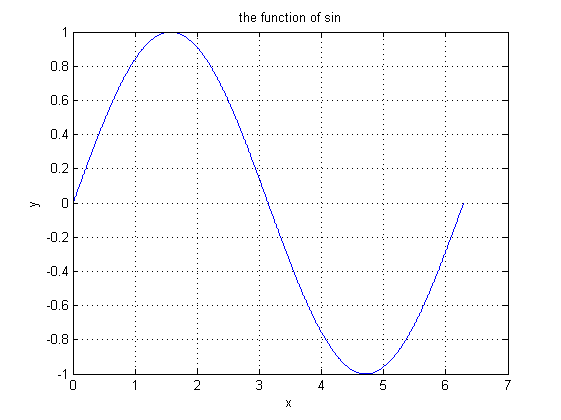
\includegraphics[scale=0.6]{sin_x}
	\caption{$ sin(x) $的函数图像}
\end{figure}
\subsubsection{Matlab的m文件}
Matlab编写的代码是以.m结尾的文件格式,m文件分为两种,m脚本文件和m函数文件。将执行的命令集写在m脚本文件中,直接在命令窗口输入文件名即可运行脚本文件,为了使文件不与Matlab自带的命令冲突,不要把文件命名与Matlab自带命令名称一致。编写脚本如下:
\begin{lstlisting}
   x = 0:0.01:2*pi;
   y = sin(x);
   plot(x,y,'-b')
   grid on
   title('the function of sin')
   xlabel('x')
   ylabel('y')\end{lstlisting}
将上面代码保存为plotsin.m文件,在命令窗口输入plotsin也可以绘制出图7函数图像。

还有一种是m函数文件,它在文件内部定义一个函数,由外界调取该函数进行计算,不可以单独运行,定义的函数名称要与文件名称一致,且不能与Matlab自带函数名称冲突。编写代码如下:
\begin{lstlisting}
 function sum = adds(x, y)
 sum = x + y;\end{lstlisting}
将上面代码保存为adds.m文件,在命令窗口输入adds(3,4),执行结果如下:
\begin{lstlisting}
 >> adds(3,4)
 	ans =
		 7\end{lstlisting}
\subsection{Matlab GUI设计}
在Matlab中,GUI设计有两种方法,一种是用代码实现界面的编程,还有一种是使用GUIDE图形界面设计,前者虽然编写代码量较大,界面的绘制都用代码实现,但在重复设计上有优势,比如大部分控件拥有相同的属性,我们可以用循环来设置。后者虽然操作简单,界面绘制布局可视化,但在控件多的情况下,重复设置属性就比较麻烦了。在本毕业设计中,采用的前种设计方法。在Matlab中图形界面的层次结构\footnote{引用参考文献[2]第9章Matlab GUI的组成与结构第183页}如下图:
\begin{figure}[H]
	\centering
	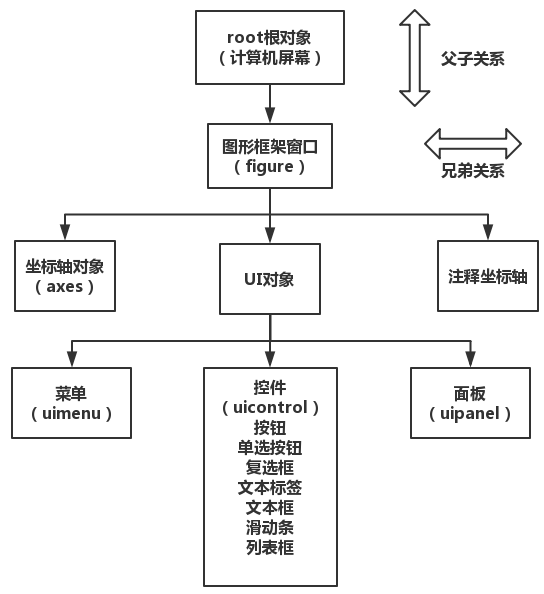
\includegraphics[scale=0.5]{MatlabGUI}
	\caption{GUI对象层次结构图}
\end{figure}
\subsubsection{Matlab中设计GUI的函数}

\subsubsection{Matlab中GUI控件的设计}
\subsubsection{Matlab中回调函数的编写}
\subsubsection{Matlab文件的读取与保存}